\chapter{Achieving the preservation of privacy}
\label{cha:3}
This chapter explains the cryptographic tools used for the problem.

\section{Cryptography or the protection of messages}
A general introduction on cryptography: history, symmetric, asymmetric, some protocols as we will use TCP channels normally.

\section{Different approaches on privacy-friendliness}
In a world of constant data exchange between different entities, it might be usefull to develop methods not only to protect data during the transit as described before, but also when in possession of an entity that should not be able to read all of it. This is of particular interest for computation outsourcing where a specific data-set has to be processed by an external entity that should not be able to infer anything more than what is asked from it. Furthermore, it might even be wished that one or more external entities might not be able to read the output of their computations, solely readable by the owner(s) of the data. This is of particular interest for the --- now everywhere --- cloud solutions. A protocol that respects the private character of data when treated by other entities than the owner is called \emph{privacy-friendly} or \emph{privacy-preserving}. There exists different approaches to privacy-friendliness and for the stake of completeness, hereafter follows a short survey of them which also justifies our choice.

\subsection{Differential privacy}
Instead of encrypting all the data, one could alternatively directly address the core problem of why we want them encrypted: to prevent other parties to get any information on what data we possess. In the case that will interest us in this thesis, we will be in possession of a lot of data from personal users which is confidential and can therefore not be traced back to the user. In 2009, Netflix launched the Neltfix prize on data recommendation: the first group to improve their recommendation score by 10\% or more would win 1.000.000\$. They provided a data-set to let the participants train their models and took care of anonymising the data before they made it accessible. However, Narayanan and Shmatikov showed how they could re-identify a lot of the users using the scores of the users on IMDb. \emph{Differential privacy} \cite{Dwork2008DifferentialResults} addresses this problem by adding noise to the data and thereby achieving a better anonymisation. In this way, the data is still usable for statistical models but cannot be used to identify anyone as easily as before. Still, differential privacy is limited by the fundamental and intrinsic relation between anonymisation and statistical relevance. One cannot obtain the first without inevitably having an influence on the second one, and reciprocally.

\subsection{Homomorphic encryption}
Differential analysis is a statistical approach of anonymity, but there exists also some cryptographic approach, where the external entity is not able to read the results of what it produces. It is possible to construct a protocol with one or more third parties in a way that they cannot possibly learn anything from what they are receiving nor what they are sending back: the information is processed in an encrypted and not a clear form. Encryption schemes that allow mathematical operations to be executed on the encrypted data are called \emph{homomorphic} and was first proposed by Rivest et al. in 1978. For example, the RSA encryption scheme preserves the multiplication over the encrypted data. As a reminder, the RSA encryption scheme is given by $\mathscr{E}(m)=m^e \mod N$. We thus have $\mathscr{E}(m_1) \cdot  \mathscr{E}(m_2) = \left(m_1^e \mod N \right)\left(m_2^e \mod N \right) = \left(m_1m_2\right)^e \mod N = \mathscr{E}(m_1m_2)$. Unfortunately, this property is only true for multiplication and is therefore quite limited in its applications. We therefore refer to RSA as a \emph{somewhat-homomorphic} encryption scheme (SHE). When all mathematical operations are possible, we say from the encryption scheme that it is \emph{fully-homomorphic} (FHE). Up to now, sole some schemes based on finite fields possess this property. 

The most accomplished method up to now is called the \emph{Approximate Eigenvector Method} and is based on the \emph{Learning With Errors} (LWE) encryption scheme, which is also known for still being secure in a post-quantum era. If $C_1$ and $C_2$ are two matrices with common eigenvector $\vec{s}$, we notice that the sum or multiplication of their respective eigenvalues $m_1$ and $m_2$ corresponds to the eigenvalue of the sum or multiplication of $C_1$ and $C_2$ with respect to $\vec{s}$. The eigenvector act as a private key and the eigenvalues as the secrect messages. The scheme is thus fully homomorphic. However, eigenvectors are easy to find and the scheme is thus also insecure. To resolve this, the method uses approximate eigenvectors $\vec{s}C=m\vec{s}+\vec{e}\approx m\vec{s}$ which is known to be still solvable in finite fields under a few assumptions about the error $\vec{e}$.

\subsection{Multi-party computation}
When different parties participate to the input, the homomorphic encryption described above cannot be used anymore: all parties have to share the same secret key which makes their data still private with respect to the third party, but not to each other. Multi-party computation address this problem. Furthermore, it also allows the parties to compute a common function on their private inputs without needing one or more third parties. 

More concretely, let us now imagine a problem where the goal is to compute some common function $f$ over private inputs $x_i$. On other words we want to compute $f\left(x_1, \, \ldots, \, x_n\right) = \left( y_1, \, \ldots , \, y_n\right)$ where each input $x_i$ is privately provided by player $i$, which ultimately learns $y_i$ and nothing more: nor the other outputs, not the other inputs. A first naive implementation would be to trust a third party for privately receiving each player's input, computing the function and privately communicating the corresponding responses to everyone. However, it also possible to obtain the same results without the trust of a third party, where the sole players are participating to the protocol. This is called \emph{multi-party computation} (MPC) also referred to as \emph{secure multi-party computation} (SMC). This approach has been chosen to solve our problem and will be now more extensively described in the next section.

\section{Multi-party computation in a nutshell}
Multi-party computation originated with the toy example presented by Yao in 1982 \cite{Yao1982ProtocolsComputations} and now known as the \emph{Millionaire's Problem}: two millionaires both want to know who is richer, but none of them want to disclose their fortune nor trust a third party. Other applications of MPC may concern electronic voting or solutions of private-data as a service (PDaaS).

+ general description of rounds etc...

\subsection{Bit-wise decomposition}
Two types: bit-wise decomposition and additive sharing. Arithmetic and boolean circuits.

\subsubsection{Oblivious transfer}
The idea behind \emph{oblivious transfer} originally described by Rabin in 1981 \cite{Rabin1981HowTransfer.} is the transfer of an information in possession of a first party and asked by a second party without the first knowing which information has been transferred. Hence, the name oblivious, or alternatively, unconscious. Different protocols exist and are all based on the \emph{RSA scheme}. 

The most common version is the \emph{1-2 oblivious transfer} \cite{Even1985AContracts} and goes as follows: Alice is in possession of two messages $m_0$ and $m_1$ and Bob wants to get message $m_p$. Alice first generates a set of private key $d$ and public key $(N,e)$ and sends two random messages $x_0$ and $x_1$ to Bob. He then generates a random message $k$ and encrypts it with the $x_i$ corresponding to the wanted message: $v = \left(x_p + k^e\right) \mod N$ and sends it to Alice. She then recovers both $k$ without knowing which one corresponds to Bob's original one: $k_i = \left(v-x_i^d\right) \mod N$. These $k_i$ then serve to encrypt the messages which are finally sent to Bob $s_i = m_i+k_i$. Bob can then only decrypt the wanted message $m_p = s_p-k$. 

This protocol has been generalised to more than two parties \cite{Ishai1997PrivateApplications,Shankar2008AlternativeTransfer,Tassa2011GeneralizedSharing}

\subsubsection{Yao's garbled circuits}
\emph{Garbled circuits} (GC) were first introduced by Yao in 1986 \cite{Yao1986HowSecrets} and now one of the most efficient solutions for generic secure two-party computation. A function has to be decomposed into a boolean circuit consisting of two-input gates (e.g. XOR and AND). Let's consider the simplest example of evaluating an AND-gate between Alice and Bob. Alice first generates a different random sequence --- also called \emph{labels} --- for each possible value of each input --- also called \emph{wires} --- and output. In the truth table, the output are then symmetrically encrypted with the hash of each corresponding input. These four resulting cyphertexts are then randomly permuted --- hence the name \emph{garbled} --- and sent to Bob. The garbling of an AND-gate is illustrated at table~\ref{tab:ang-garb}. Once Bob receives the garbled gate, he then asks Alice for her label. As they have been randomly chosen, she can send it to him without him possibly knowing what value it corresponds to. Afterwards, he also needs to know the label of his input. This part is a bit more tricky and is solved using the previously described \emph{oblivious transfer}. Bob can now compute the hash of the two labels and decrypt each element of the garbled gate until we find one corresponding with the garbled gate he recieved from Alice. He can then reveal the value to Alice either she can reveal the mapping of the garbling. The same principle can be used on a multi-gate circuit by garbling the sole end result.

\begin{figure}
        \begin{subfigure}[b]{.32\textwidth} 
            \centering 
            \begin{tabular}{IC{.6cm}|C{.6cm}IC{1.3cm}I}
            \hlineI
            A & B & output \\ \hlineI
            0 & 0 & 0  \\ \hline
            1 & 0 & 0 \\ \hline
            0 & 1 & 0 \\ \hline
            1 & 1 & 1 \\ \hlineI
            \end{tabular}
            \caption{Truth table.} 
        \end{subfigure}
        \hfill
        \begin{subfigure}[b]{.32\textwidth} 
            \centering 
            \begin{tabular}{IC{.6cm}|C{.6cm}IC{1.3cm}I}
            \hlineI
            A & B & output \\ \hlineI
            $x_A^0$ & $x_B^0$ & $x_{\textnormal{output}}^0$ \\ \hline
            $x_A^1$ & $x_B^0$ & $x_{\textnormal{output}}^0$ \\ \hline
            $x_A^0$ & $x_B^1$ & $x_{\textnormal{output}}^0$ \\ \hline
            $x_A^1$ & $x_B^1$ & $x_{\textnormal{output}}^1$ \\ \hlineI
            \end{tabular}
            \caption{Labelled truth table.} 
        \end{subfigure}
        \hfill
        \begin{subfigure}[b]{.32\textwidth}
            \centering 
            \begin{tabular}{IC{3.2cm}I}
            \hlineI
            output \\ \hlineI
            $\mathscr{E}_{H\left(x_A^1,x_B^0\right)}\left(x_{\textnormal{output}}^0\right)$ \\ \hline
            $\mathscr{E}_{H\left(x_A^1,x_B^1\right)}\left(x_{\textnormal{output}}^1\right)$ \\ \hline
            $\mathscr{E}_{H\left(x_A^0,x_B^0\right)}\left(x_{\textnormal{output}}^0\right)$ \\ \hline
            $\mathscr{E}_{H\left(x_A^0,x_B^1\right)}\left(x_{\textnormal{output}}^0\right)$ \\ \hlineI
            \end{tabular}
            \caption{Garbled output.} 
        \end{subfigure}
        \captionof{table}{Garbling of the AND-gate.}
        \label{tab:ang-garb}
\end{figure}

It is interesting to note that the secure evaluation of a sole AND-gate does not respect the principles of the multi-party computation, by definition of the AND-gate. Indeed, if the final solution is 1, both players know their respective input value, which is thus disclosed\footnote{This is not the case for the XOR-gate as an 1-output has two corresponding inputs possible, as has the 0-output}. Therefore, the total functions evaluated have to be totally surjective for each input. The circuit corresponding to the Millionaire's problem is given at figure~\ref{c2:yao-comp} and while it consists of AND-gates, the function is totally subjective with respect to each millionaire's fortune.

\begin{figure}[ht!]
    \centering
    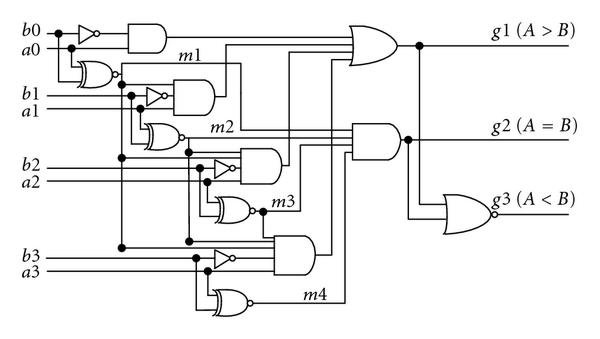
\includegraphics[width=.7\textwidth]{parts/chap-3/img/yao-comp.jpg}
    \caption{The figital comporator is the boolean circuit used to soleve Yao's millionnaire problem.} 
    \label{c2:yao-comp}
\end{figure}

This protocol executes in polynomial time, but there exists a lots of optimisations that allow to garble and evaluate the gates more rapidly.

\subsubsection{GMW protocol}
The \emph{Goldreich-Micali-Widgerson} (GMW) protocol can be seen as an extension of garbled circuits to multiple parties using Yao's idea of using oblivious transfer \cite{Goldreich1987HowGame}. The main principles here are based upon bit-sharing: each party shares its input bits among the $n$ players $b = \sum_{i=1\ldots n}b_i \mod 2$. Each player then processes their shares among the circuit. XOR-gates are easy as they can just addition the shares $c_i = a_i + b_i$. However AND-gates are more tricky: we can see from the decomposition that $c = a \cdot b = \sum_{i\neq j}a_ib_j+\sum_{1\leq i< j\neq n}\left(a_ib_j + a_jb_i \right) \mod 2$. By consequence, each party will have to compute $a_ib_i+ \sum_{i\neq j}\left( a_ib_j + a_jb_i\right)$. As for the XOR-gate, the first part is trivial to evaluate, however, the second cannot be computed by party $i$ without more information from party $j$. This is solved by using a variant of garbled circuits with oblivious transfer between parties $i$ and $j$.

\subsection{Avoiding bit-wise decomposition}
Alternatively, some arithmetic circuits can also be used for multi-party computation. The problem of the bit-wise decomposition and the use of the boolean circuit transcription of the function we jointly want to evaluate is their expensiveness in terms of performance. Indeed, a simple operation can rapidly lead to a lot of gates. For example, let's consider the addition of two number: for two numbers of $n$ bits, the total number of gates is $5n$ in a full adder composition. This is even worse for multiplication. Of course, some optimisations can be made, but the general number of gates is very high compared to the arithmetic circuit of the same function, where it would just be one single gate for addition and multiplication. We will see later that MPC over arithmetic circuits has a much higher \emph{round complexity} --- the dependence of the different rounds on each other --- which leads to less possible parallelisation than with boolean circuits. Nevertheless, one can argue that the parallelisation of bit-wise decomposition does not compensate the much higher number of gates and is thus less efficient than arithmetic circuits in general \cite{Aly2018PracticallyBit-Decomposition}.

+ general comparison of bit-wise decomposition performance and additive secret sharing comparison \cite{Blom2014AThesis}.

Comparisons are much more feasible in boolean circuits.

\subsubsection{How to share a secret}
The building block of multi-party computation over arithmetic is based upon secret sharing. Each party computes its own version of the circuit with the shares of the different parties. At the end of the circuit processing, each party has a share of the final output, which can then be put together to obtain the final output. We first have to define a way for a party to share its secret among $n$ parties, including itself.

\paragraph{Additive secret sharing}
The simplest idea is just to divide the secret $a$ in $n$ shares $a_i$ using a simple summation: $a = \sum_{i=1 \ldots n}a_i$. However, doing it in this manner allows the shares to release some information about the secret, as the shares are not random and strongly depend on the secret. They are two solutions to this problem and the first one is to consider additive sharing over $\mathbb{Z}_q$. The sharing now becomes $a = \sum_{i=1\ldots n}a_i \mod q$ which solves the problem, as the shares can now really be chosen at random. The other solution is over $\mathbb{Z}$ and consists in choosing a sufficiently large interval in which the shares are chosen to dilute sufficiently the statistical information about the secret, typically $a_i \in \left[-A2^\rho,A2^\rho\right]$ with $A$ the size of the interval of the secret $a \in \left[-A,A\right]$ and typically $\rho=128$.

Another consequence of this scheme is that all parties are vital to the recovery of secret as a loss of one secret unables us to reconstruct the secret or any statistical information about it as we took care of that. The scheme does not tolerate the loss or treason of one party and is therefore very sensitive to any failure or malicious player. This problem is solved by polynomial secret sharing.



\paragraph{Polynomial secret sharing}
The idea of polynomial sharing was originally proposed by Shamir in 1979 \cite{Shamir1979HowSecret}. This method allows $n$ parties to share a secret in a way such that any subset of $t+1$ parties can later reconstruct the secret but any subgroup of maximum $t$ parties can do so. The scheme is based on the single fact that for any polynomial of degree $d$, any subset of $d+1$ or more different points can reconstruct the polynomial completely whereas any subset of at most $d$ points is left with an infinite number of possibilities.

The scheme goes as follows. The party that wants to share its secret first constructs a polynomial of degree $t$.
\begin{equation}
    h(z) = a + \sum_{i=1}^t b_i z^i
\end{equation}
with secret $a$ random coefficients $b_i$. For the same reasons as for additive secret sharing, the coefficients can either be chosen in $b_i \in \mathbb{Z}_q$ (which also leads to the consideration of polynomial $h(z) \mod q$ instead), either in the interval $b_i \in \left[-A2^\rho,A2^\rho\right]$.
\noteH{should I demonstrate ?}

We verify that $h(0)=a$ and distribute shares $a_i$ to each party $i$ --- including ourselves --- as follows $a_i=h(i)$. $t+1$ parties can now reconstruct the polynomial together using e.g. Lagrange's polynomials and compute $f(0)$ to recover the secret share. An interesting property is that the recovery can be done as a simple linear combination. Indeed, we have
\begin{eqnarray*}
    h(0) &=& \sum_{i=1}^{n} l_i(0)h(i) \\
    a &=& \sum_{i=1}^{n} r_ia_i
\end{eqnarray*}
where $r = \left(r_1, \ldots , r_n\right) = \left(l_1(0), \ldots , l_n(0)\right)$ is called the \emph{recombination vector} with $l_i(z)$ the $i$-th order Lagrange polynomial, for example
\begin{equation*}
    l_i(z) = \prod_{1\leq j \leq n,j\neq i}\frac{z-j}{i-j}
\end{equation*}
This also works with any generating set of $\mathbb{Z}\left[z\right]$ (or alternatively $\mathbb{Z}_q\left[z\right]$), as long all parties use the same set.

\subsubsection{Performing basic operations}

\paragraph{Addition and multiplication of public constants}
Each party just adds or multiplies his share with the constant. This rests on some arithmetic properties of polynomials: one can easily verify that $a_i+c$ is a share of $a+c$ and $c \cdot a_i$ of $c \cdot a$.

\paragraph{Addition of two secrets}
Let's consider the addition of two polynomials: the respective coefficients just add up. By consequence, two secrets $a$ and $b$ can be added up if every party adds their local shares $a_i+b_i$.
\noteH{False, the values $h(i)$ are added up, not the coefficients}


\paragraph{Multiplication of two secrets}
Unfortunately, it is not possible to adopt the same strategy for multiplication as the multiplication of two polynomials of order $t$ will lead to a new polynomial of order $2t$ which will double the number of parties needed to recover the secret output. In real-case functions with a lot of multiplications, this becomes rapidly impracticable and theoretically unsolvable if the degree of the new polynomial exceeds $n$. Another problem is of statistical order: the new polynomial is not random anymore as it is for example not irreducible anymore by construction. Different algorithms exist to solve this problem \noteH{cite different algorithms ?}

\paragraph{Exponentiation}


\paragraph{Boolean operations}


\section{Security of the model}
Semi-honest model + some explanations obout the active case.


\subsection{Passive case}



\subsection{Active case}


\section{Key performance indicators}
Now that we know when a comparison protocol is secure in the Semi honest model, we should discuss when such protocols are considered “good”. This will not be done by defining a single attribute to be good, rather we pick key performance indicators (KPI) so we get a transparent view of the performance different protocols might display in different settings.

\subsection{Communication Complexity}
The total communication needed by a protocol can be measured by the number of Kilo Bytes (KB) of data which have to be send over a communication line during a protocol. Obviously, a protocol which enforces 1 GB = 10242 KB of communication is not considered a good protocol when compared to another protocol which only needs 100 KB of communication data. Usually, the communication performance of a protocol depends greatly on the bit-length of the input. So in order to keep the performance evaluation fair, one should make sure to optimize the total communication as good as possible considering a given input length ? for the protocol.

\subsection{Round Complexity}
In many applications, the number of communication rounds tends to be the bottle neck of a protocol. This is due to the fact that a lot of overhead capacity might be needed to initiate and terminate a (secure) communication line between the other party. In general, however, this really depends on the communication technology used in practise. We use Toft’s definition of a round of communication, because it gives us a workable and intuitive definition of this concept. Toft argues that a communication round consists of sending information to other parties and performing a limitless number of arithmetic computations with a sole restriction: variables which are received by a party during this round can not be used in any arithmetic operation performed by that party in the same round.

\subsection{Bandwidth}
The bandwidth of a protocol is given by the maximum number of bits send during a single communication round. This performance indicator strikes an interesting issue consider the previous two KPI. When the communication complexity of a protocol doesn’t change, but we manage to decrease the round complexity, then odds are that the necessary bandwidth for the protocol will increase. This is obviously not always the case, but shows that we might encounter some trade off considering these KPI. Note that when one finds the necessary bandwidth of a protocol to hight in practise, one can always implement the rounds with the highest communication complexity complexity as two separate communications to decrease the bandwidth.

\subsection{Computational Complexity}
This KPI is mentioned way less in recent literature than the previous ones. Which is one of the main reasons why this research project exists in the first place. The Computational complexity is measured as the amount of time it takes ones CPU to compute the desired result of a protocol. This KPI is shunned so often as it takes a lot of extra time and effort to implement the proposed protocol. To our knowledge, the only secure comparison protocol, described in the next chapter, for which the computation complexity was studied previous to our research, was that of Garbled Circuits.
